% !TEX encoding = UTF-8
% !TEX TS-program = pdflatex
% !TEX root = ../tesi.tex

%**************************************************************
\chapter{Applicazione}
\label{cap:applicazione}

%**************************************************************
\section{Analisi}

\subsection{Descrizione}

Durante la prima parte dello stage, svolgendo le attività di studio e formazione personale sul contesto aziendale e sulla \gls{blockchaing} sviluppata da Commerc.io S.r.l., sono stati individuati i temi di principale interesse per \myCompany{} \companyTitle:

\begin{itemize}
	\item la gestione delle identità digitali e delle informazioni che le caratterizzano;
	\item lo scambio di documenti con valore legale associati ad un'identità tramite la relativa firma elettronica.
\end{itemize}

Di conseguenza, l'obiettivo principale della seconda fase del progetto è stato realizzare un prototipo che dimostrasse la fattibilità dell'implementazione di un'applicazione per dispositivi mobili inerente alle due precedenti tematiche. Questa doveva permettere agli utenti di registrare una propria \gls{ssi} e, una volta completata l'apposita procedura, di utilizzarla per certificare la paternità degli eventuali documenti caricati e poi condivisi con altri utenti, tramite il programma stesso.\\
L'applicazione dovrà essere disponibile sia per dispositivi Android che per dispositivi iOS, mantenendo un'interfaccia grafica il più coerente e simile possibile, indipendentemente dal sistema operativo su cui veniva eseguita, e fornendo le stesse funzionalità. In particolare, ogni utente dovrà poter:

\begin{itemize}
	\item registrare una nuova identità, la quale sarà poi accessibile ed utilizzabile solamente all'interno del sistema attualmente utilizzato;
	\item recuperare un'identità precedentemente creata in un dispositivo differente da quello corrente;
	\item accedere alla propria identità in modo sicuro;
	\item utilizzare l'identità all'interno dell'applicazione per effettuare le diverse operazioni messe a disposizione.
\end{itemize}

Le prime tre funzionalità richiederanno l'esecuzione di alcune operazioni che, poste in una sequenza ordinata, andranno a formare una procedura che dovrà essere seguita passo passo per poter raggiungerne lo scopo.\\\\
Per registrare una nuova identità sarà necessario inserire il proprio nome e cognome e scegliere il metodo di autenticazione desiderato tra quelli disponibili, ossia \textit{password} alfanumerica o dati biometrici; nel caso venga fatta la prima scelta verrà richiesto l'inserimento, con successiva conferma, della \textit{password} desiderata, altrimenti sarà necessario autenticarsi con l'impronta digitale o con l'identificativo facciale prima di poter proseguire. Successivamente verrà chiesto di inserire il proprio indirizzo di posta elettronica e, una volta confermato, un codice di verifica numerico inviato all'utente tramite \textit{email} per certificare l'effettiva proprietà della casella indicata. La stessa operazione dovrà essere poi ripetuta per l'inserimento del numero di telefono cellulare, in questo caso la verifica verrà effettuata tramite \gls{sms}\glsfirstoccur. Infine verrà generato e visualizzato a schermo il codice mnemonico usato per generare il \gls{walletg} associato alla \gls{ssi} appena creata, e sarà possibile salvarlo in formato \gls{pdf}\glsfirstoccur{} all'interno della memoria del dispositivo, oppure stamparlo direttamente dall'applicazione. È di vitale importanza far capire all'utente che non deve smarrire questo codice, in quanto è l'unica informazione utilizzabile per ripristinare l'accesso alla propria identità.\\\\
Per poter recuperare una vecchia identità ed accedervi con un nuovo dispositivo, diverso da quello utilizzato per crearla la prima volta, verrà prima richiesto il metodo di autenticazione desiderato, allo stesso modo della procedura di registrazione e, dopo aver fornito i dati necessari, dovrà essere inserito il codice mnemonico generato durante la creazione della \gls{ssi}. Solo nel caso questo sia corretto l'utente potrà accedere alla propria identità, altrimenti la procedura terminerà con un'errore e, per poter utilizzare l'applicazione, sarà quindi indispensabile ripetere nuovamente il procedimento di registrazione dall'inizio.\\\\
Per effettuare l'accesso, invece, non sarà necessario inserire il codice mnemonico, ma sarà sufficiente fornire i dati di autenticazione richiesti in base al metodo scelto in precedenza. Se era stato selezionato il riconoscimento biometrico, allora l'utente dovrà utilizzare la propria impronta digitale o il riconoscimento facciale per entrare, altrimenti verrà richiesto l'inserimento della \textit{password} alfanumerica scelta dall'utente durante la registrazione.\\\\
Una volta all'interno dell'applicazione, le funzionalità che saranno a disposizione dell'utente sono:

\begin{itemize}
	\item visualizzazione della foto e delle informazioni associate alla propria identità, corredate dall'indirizzo pubblico e dal bilancio del \gls{walletg} ad essa associato;
	\item visualizzazione della foto, del nome e delle informazioni associate ad ogni documento inserito all'interno dell'applicazione;
	\item visualizzazione del codice QR associato all'indirizzo pubblico del proprio \gls{walletg};
	\item inserimento di una nuova foto profilo, la quale può essere scattata direttamente all'interno dell'applicazione;
	\item inserimento di un nuovo documento.
\end{itemize}

\subsection{Requisiti}

L'obiettivo principale che si desidera raggiungere è l'implementazione di un \gls{poc} che dimostri la fattibilità dell'applicazione d'interesse per l'azienda, di conseguenza il progetto non prevede uno sviluppo \textit{software} completo, ma limitato a rendere disponibili le operazioni più significative. Quindi, dopo un'attenta analisi del problema proposto e delle funzionalità richieste per l'applicazione, tenendo anche conto del tempo rimasto a disposizione per il progetto di stage, sono stati individuati diversi tipi di requisiti, in base all'importanza e alla quantità di lavoro richiesta per riuscire a soddisfarli.\\
Per identificare ogni requisito in modo univoco si è fatto utilizzo di un opportuno codice, il quale è strutturato nel modo seguente:\\

\begin{center}
	\textbf{R[T][P]-[N]}
\end{center}

Dove ogni lettera ha un preciso significato:

\begin{itemize}
	\item \textbf{R:} requisito;
	
	\item \textbf{T:} tipologia, differisce in base allo specifico requisito e può assumere i seguenti valori:
		\begin{itemize}
			\item \textbf{F:} funzionale, ossia un requisito che indica una caratteristica operativa che il \textit{software} deve avere;
			\item \textbf{Q:} qualitativo, ossia un requisito che indica una caratteristica, non necessariamente legata al \textit{software}, ma che ne aumenta la qualità in termini di efficacia ed efficienza;
			\item \textbf{V:} vincolo, ossia un requisito che indica una caratteristica, non necessariamente legata al \textit{software}, ma che deve essere garantita su richiesta dell'azienda;
		\end{itemize}
	
	\item \textbf{P:} priorità, differisce in base allo specifico requisito e può assumere i seguenti valori:
		\begin{itemize}
			\item \textbf{O:} obbligatorio, ossia un requisito vincolante in quanto primario e fondamentale;
			\item \textbf{D:} desiderabile, ossia un requisito non vincolante o strettamente necessario, ma dal riconoscibile valore aggiunto;
			\item \textbf{F:} funzionale, ossia un requisito rappresentante valore aggiunto non strettamente competitivo; 
		\end{itemize}
	
	\item \textbf{N:} numero, intero progressivo maggiore di zero con funzione di identificativo del requisito.
\end{itemize}

Di seguito vengono riportati tutti i requisiti riguardanti lo sviluppo del \gls{poc}, suddivisi in tre tabelle, una per ogni tipologia.

\rowcolors{1}{grayer}{white}
\begin{longtable}{|c|p{10.5cm}|}
	\hline
	\rowcolor{gray}
	\textbf{Requisito} & \textbf{Descrizione} \\
	\hline
	RFO-1     & L'applicazione deve permettere l'inserimento del nome dell'utente. \\
	\hline
	RFO-2     & L'applicazione deve permettere l'inserimento del cognome dell'utente. \\
	\hline
	RFO-3     & L'applicazione deve permettere l'inserimento dell'indirizzo di posta elettronica dell'utente. \\
	\hline
	RFO-4     & L'applicazione deve permettere l'inserimento del numero di telefono cellulare dell'utente. \\
	\hline
	RFO-5     & L'applicazione deve permettere l'inserimento del codice di verifica dell'indirizzo di posta elettronica dell'utente. \\
	\hline
	RFO-6     & L'applicazione deve permettere l'inserimento del codice di verifica del numero di telefono cellulare dell'utente. \\
	\hline
	RFO-7     & L'applicazione deve permettere l'invio del codice di verifica dell'indirizzo di posta elettronica dell'utente. \\
	\hline
	RFO-8     & L'applicazione deve permettere l'invio del codice di verifica del numero di telefono cellulare dell'utente. \\
	\hline
	RFO-9     & L'applicazione deve permettere la visualizzazione del codice mnemonico. \\
	\hline
	RFO-10    & L'applicazione deve permettere l'inserimento del codice mnemonico. \\
	\hline
	RFO-11    & L'applicazione deve permettere l'inserimento di una \textit{password} per l'accesso da parte dell'utente. \\
	\hline
	RFO-12    & L'applicazione deve permettere l'inserimento della \textit{password} di accesso dell'utente. \\
	\hline
	RFO-13    & L'applicazione deve permettere la scelta dell'accesso tramite \textit{password} da parte dell'utente. \\
	\hline
	RFO-14    & L'applicazione deve permettere l'inserimento della password per l'accesso da parte dell'utente. \\
	\hline
	RFO-15    & L'applicazione deve permettere la visualizzazione del nome dell'utente. \\
	\hline
	RFO-16    & L'applicazione deve permettere la visualizzazione del cognome dell'utente. \\
	\hline
	RFO-17    & L'applicazione deve permettere la visualizzazione dell'indirizzo di posta elettronica dell'utente. \\
	\hline
	RFO-18    & L'applicazione deve permettere la visualizzazione del numero di telefono cellulare dell'utente. \\
	\hline
	RFO-19    & L'applicazione deve permettere la visualizzazione dell'indirizzo pubblico del \gls{walletg} dell'utente. \\
	\hline
	RFO-20    & L'applicazione deve permettere la visualizzazione del saldo del \gls{walletg} dell'utente. \\
	\hline
	RFO-21    & L'applicazione deve permettere la visualizzazione della foto profilo dell'utente. \\
	\hline
	RFO-22    & L'applicazione deve permettere la visualizzazione della lista dei documenti inseriti dall'utente. \\
	\hline
	RFO-23    & L'applicazione deve permettere la registrazione di una nuova identità da parte dell'utente. \\
	\hline
	RFO-24    & L'applicazione deve permettere il recupero di un'identità creata in precedenza da parte dell'utente. \\
	\hline
	RFO-25    & L'applicazione deve permettere l'accesso tramite autenticazione da parte dell'utente. \\
	\hline
	RFD-1     & L'applicazione deve permettere il reinvio del codice di verifica dell'indirizzo di posta elettronica dell'utente. \\
	\hline
	RFD-2     & L'applicazione deve permettere il reinvio del codice di verifica del numero di telefono cellulare dell'utente. \\
	\hline
	RFD-3     & L'applicazione deve permettere il salvataggio del codice mnemonico in formato \gls{pdf}. \\
	\hline
	RFD-4     & L'applicazione deve permettere la scelta dell'accesso tramite dati biometrici da parte dell'utente. \\
	\hline
	RFD-5     & L'applicazione deve permettere l'inserimento dei dati biometrici per l'accesso da parte dell'utente. \\
	\hline
	RFD-6     & L'applicazione deve permettere l'inserimento della foto profilo da parte dell'utente. \\
	\hline
	RFD-7     & L'applicazione deve permettere l'inserimento del titolo di un documento da parte dell'utente. \\
	\hline
	RFD-8     & L'applicazione deve permettere l'inserimento delle informazioni di un documento da parte dell'utente. \\
	\hline
	RFD-9     & L'applicazione deve permettere l'inserimento di un documento da parte dell'utente. \\
	\hline
	RFF-1     & L'applicazione deve permettere la stampa del codice mnemonico. \\
	\hline
	RFF-2     & L'applicazione deve permettere la visualizzazione del codice QR associato all'indirizzo pubblico del \gls{walletg}. \\
	\hline
	RFF-3     & L'applicazione deve permettere la modifica della foto profilo da parte dell'utente. \\
	\hline
	RFF-4     & L'applicazione deve permettere l'inserimento della foto di un documento da parte dell'utente. \\
	\hline
	
	\caption{Tabella dei requisti funzionali}
	\label{tab:requisiti-funzionali}
\end{longtable}

\rowcolors{1}{white}{grayer}
\begin{longtable}{|c|p{10.5cm}|}
	\hline
	\rowcolor{gray}
	\textbf{Requisito} & \textbf{Descrizione} \\
	\hline
	RQO-1    & Deve essere fornita una documentazione delle procedure di installazione e configurazione di tutte le tecnologie e gli strumenti utilizzati per sviluppare e testare l'applicazione. \\
	\hline
	RQO-2    & Deve essere fornita una documentazione di tutte le classi che compongono l'applicazione, con i relativi metodi. \\
	\hline
	RQO-3    & Il processo di sviluppo deve fare uso di un sistema di versionamento. \\
	\hline
	
	\caption{Tabella dei requisiti qualitativi}
	\label{tab:requisiti-qualitativi}
\end{longtable}

\rowcolors{1}{white}{grayer}
\begin{longtable}{|c|p{10.5cm}|}
	\hline
	\rowcolor{gray}
	\textbf{Requisito} & \textbf{Descrizione} \\
	\hline
	RVO-1    & L'applicazione deve essere scritta utilizzando il linguaggio Dart. \\
	\hline
	RVO-2    & L'applicazione deve essere scritta utilizzando il \gls{frameworkg} Flutter. \\
	\hline
	RVO-3    & L'applicazione deve interagire con la \gls{blockchaing} della \textit{Commercio.network}. \\
	\hline
	RVO-4    & L'interazione a basso livello con la \gls{blockchaing} deve avvenire tramite la libreria Sacco, sviluppata da Commerc.io S.r.l. per il linguaggio di programmazione Dart. \\
	\hline
	RVO-5    & L'interazione ad alto livello con la \gls{blockchaing} deve avvenire tramite la libreria CommercioSDK, sviluppata da Commerc.io S.r.l. per il linguaggio di programmazione Dart. \\
	\hline
	RVO-6    & L'applicazione deve essere eseguibile su sistema operativo Android. \\
	\hline
	RVD-1    & L'applicazione deve essere eseguibile su sistema operativo iOS. \\
	\hline
	
	\caption{Tabella dei requisiti di vincolo}
	\label{tab:requisiti-vincolo}
\end{longtable}
	

%**************************************************************
\section{Progettazione}

Per la progettazione delle classi utilizzate nel prodotto sono stati creati degli appositi diagrammi.\\
I diagrammi delle classi sono diagrammi di tipo \gls{uml}\glsfirstoccur{} dedicati alla rappresentazione dei campi dati e dei metodi offerti da ogni classe del sistema. Tuttavia, lo scopo principale è mostrare le relazioni di dipendenza che sussistono tra le classi stesse, in modo da fornire un'idea delle interazioni presenti all'interno del sistema.\\
Essendo il progetto finalizzato alla creazione di un'applicazione per dispositivi mobili, la maggior parte delle classi previste servono per l'implementazione dell'interfaccia grafica, in quanto ognuna di esse realizza una singola schermata. Di conseguenza, le uniche classi che presentano interazioni non banali, e quindi utili da rappresentare, sono quelle che implementano la logica applicativa. Viene quindi riportato solamente il diagramma delle classi presenti nel \gls{namespaceg}\glsfirstoccur{} denominato \textit{model} che contiene tutte le funzionalità inerenti alla logica di \textit{business}.

\subsection{Logica applicativa}

La logica applicativa comprende tutte le funzionalità necessarie per la comunicazione tra l'interfaccia grafica e le strutture dati sottostanti, consentendo sia il corretto flusso di dati tra le due parti, che l'elaborazione dei dati stessi in base allo scopo della specifica operazione eseguita dell'applicazione.\\
All'interno del \gls{poc}, la logica applicativa avrà il compito di ricevere dall'interfaccia grafica i comandi che impartisce l'utente che la sta utilizzando e di eseguire, in risposta, le operazioni corrispondenti sulla \gls{blockchaing}, dandone poi prova tangibile a schermo. Quindi sarà responsabile dell'implementazione di tutte le funzionalità offerte dall'applicazione tramite la \gls{blockchaing}.\\
Per fare ciò sfrutterà la \gls{sdk}\footcite{manual:sdk-commercio-network} sviluppata da Commerc.io S.r.l., la quale fornisce tutte le classi e tutti i metodi di base necessari per realizzare operazioni più complesse e utili per degli scopi applicativi. In particolare verranno utilizzati i seguenti moduli:

\begin{itemize}
	\item \textbf{Commercio \textit{Account}:} fornisce una classe Wallet che comprende le funzionalità di creazione e recupero di un \gls{walletg} tramite l'apposito codice mnemonico, inoltre dispone di apposti metodi per la gestione sicura e il salvataggio del codice stesso. Oltre a questo, incapsula le funzionalità di richiesta e di invio di \gls{tokeng} a \gls{walletg} di altri utenti sulla \gls{blockchaing} e permette anche di controllare il proprio bilancio attuale. 
	\item \textbf{Commercio \textit{ID}:} fornisce una classe IdHelper che comprende le funzionalità per creare, gestire ed utilizzare un \gls{did} e tutti i relativi \gls{ddo} ad esso associati. Inoltre dispone di appositi metodi per effettuare delle richieste di \gls{power-upg} nei confronti di altri \gls{did} paritari.
	\item \textbf{Commercio \textit{Docs}:} fornisce una classe DocsHelper che comprende le funzionalità per condividere dei documenti con altri utenti e per inviare una conferma di avvenuta ricezione di un documento recapitato tramite la \gls{blockchaing}. Inoltre dispone di appositi metodi per reperire la lista di tutti i documenti condivisi e ricevuti, e di tutte le conferme di avvenuta ricezione inviate e recepite.
\end{itemize} 

\begin{figure}[!h] 
	\centering 
	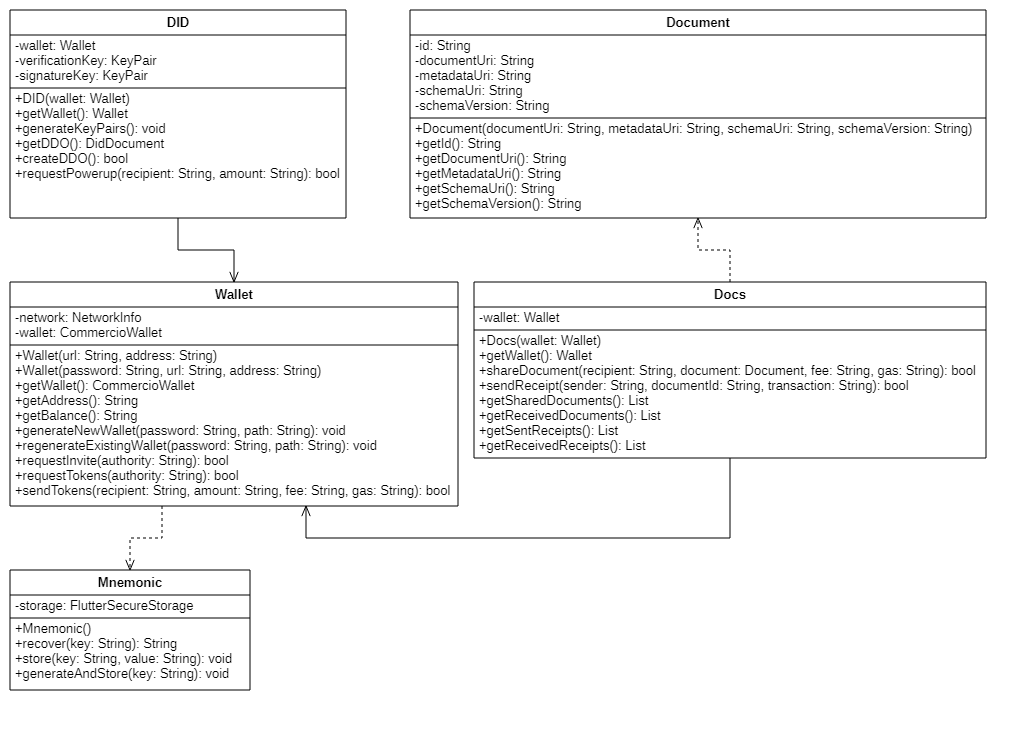
\includegraphics[width=1.04\columnwidth]{model-classes-diagram} 
	\caption{Diagramma delle classi del \gls{namespaceg} \textit{model}}
\end{figure}

\begin{namespacedesc}
    \classdesc{Database}{la classe Database incapsula un'istanza della classe sqflite.Database per l'interazione con un \textit{database} SQLite. Al suo interno sono implementati i metodi per l'inizializzazione della tabella contenente il metodo di autenticazione scelto dall'utente, con l'eventuale \textit{password}, per l'aggiunta di un nuovo metodo di autenticazione, per il controllo della presenza di uno specifico metodo e per il reperimento di tale metodo.}
    
    \classdesc{DID}{la classe DID incapsula un'istanza della classe Wallet e due coppie di chiavi crittografiche per la firma delle operazioni effettuate tramite la classe stessa. Al suo interno sono implementati i metodi per il reperimento e la creazione di un \gls{ddo} associato al \gls{did} rappresentato dal \gls{walletg} e per effettuare una richiesta di \gls{power-upg} verso il proprietario di un altro \gls{walletg}.}
    
    \classdesc{Docs}{la classe Docs incapsula un'istanza della classe Wallet per la realizzazione delle funzionalità che fornisce. Al suo interno sono implementati i metodi per la condivisione di un documento con un proprietario di un \gls{walletg}, per l'invio di una conferma di avvenuta ricezione in risposta ad un documento ricevuto in precedenza e per il reperimento della lista di tutti i documenti inviati/ricevuti e di tutte le conferme di avvenuta ricezione inviate/ricevute.}
    
    \classdesc{Document}{la classe Document rappresenta un documento che può essere condiviso attraverso la classe Docs. Essa è caratterizzata da un identificativo univoco, il riferimento al contenuto del documento, il riferimento ai meta-dati del documento, il riferimento dello schema del documento e la relativa versione.}
    
    \classdesc{Mnemonic}{la classe Mnemonic incapsula un'istanza della classe FlutterSecureStorage per l'interazione con lo spazio di archiviazione sicuro del dispositivo. Al suo interno sono implementati i metodi per la scrittura e la lettura del codice mnemonico necessario per la generazione di un \gls{walletg}.}
    
    \classdesc{Wallet}{la classe Wallet incapsula un'istanza della classe sacco.Wallet per la realizzazione di tutte le funzionalità legate ad un \gls{walletg} della rete \textit{Commercio.network}. Al suo interno sono implementati i metodi per la generazione e il recupero di un \gls{walletg}, per il reperimento dell'indirizzo pubblico e del saldo di un \gls{walletg}, per la richiesta di invito alla rete e per la richieste e l'invio di \gls{tokeng} tramite la \gls{blockchaing}.}
\end{namespacedesc}

\subsection{Interfaccia grafica}

L'interfaccia grafica comprende tutte le funzionalità necessarie per collegare le azioni compiute dall'utente alla logica applicativa, consentendo sia il corretto flusso di dati tra le due che l'elaborazione dei dati stessi in base allo scopo dell'operazione eseguita dell'applicazione, ma anche la visualizzazione dell'esito dell'operazione da parte dell'utente.\\
All'interno del \gls{poc}, l'interfaccia grafica avrà il compito di presentare all'utente che la sta utilizzando tutte le funzionalità rese disponibili dall'applicazione, in modo semplice ed efficace, utilizzando solamente i componenti strettamente necessari, così da assicurare la massima comprensibilità e facilità d'utilizzo. Quindi sarà responsabile dell'implementazione di tutto il \textit{layout} grafico dell'applicazione.\\
Per fare ciò sfrutterà il \gls{frameworkg} Flutter, il quale fornisce tutte le classi e tutti i metodi di base necessari per realizzare componenti grafici più complessi e utili per degli scopi applicativi. In particolare verranno sviluppate le seguenti sezioni principali:

\begin{itemize}
	\item \textbf{\textit{Home}:} comprende tutte le schermate che espongono le funzionalità fornire dall'applicazione all'utente che la utilizza.
	\item \textbf{\textit{Login}:} comprende tutte le schermate che espongono le funzionalità necessarie all'utente per accedere all'interno dell'applicazione.
	\item \textbf{\textit{Recover}:} comprende tutte le schermate che espongono le funzionalità necessarie all'utente per recuperare l'accesso ad un'identità precedentemente create utilizzando un diverso dispositivo mobile, in modo da poterla usare nuovamente all'interno dell'applicazione.
	\item \textbf{\textit{Registration}:} comprende tutte le schermate che espongono le funzionalità necessarie all'utente per registrare una nuova identità digitale da utilizzare all'interno dell'applicazione per effettuare le operazioni messe a sua disposizione.
\end{itemize}

\begin{namespacedesc}
	\classdesc{App}{la classe App implementa un componente grafico senza mantenimento di stato che incapsula un oggetto di classe MaterialApp, questo a sua volta contiene un'istanza del componente grafico che implementa la schermata attualmente visualizzata sullo schermo del dispositivo durante l'esecuzione dell'applicazione.\\
	Oltre a ciò, implementa un metodo per l'istanziazione del componente grafico corretto sulla base della rotta specificata durante la navigazione che effettua l'utente utilizzando l'applicazione. A questo scopo definisce anche le costanti che rappresentano le singole rotte di ogni componente grafico che implementa una schermata dell'applicazione, queste sono accessibili da ogni altra classe per permettere ad ognuna di esse di implementare dei propri metodi per la navigazione tra pagine adiacenti.}

	\classdesc{Header}{la classe Header implementa un componente grafico senza mantenimento di stato con un titolo parametrico e un'icona. Viene istanziato da ogni componente grafico che implementa una schermata dell'applicazione, il quale lo utilizza per standardizzare l'intestazione dell'applicazione stessa.}
\end{namespacedesc}

\subsubsection*{Home}

In questo \gls{namespaceg} sono raggruppate tutte le classi utilizzate per la realizzazione delle schermate che espongono le funzionalità fornite dall'applicazione una volta effettuata la registrazione ed eseguito l'accesso da parte dell'utente.

\begin{namespacedesc}
	\classdesc{Contact}{la classe Contact implementa un componente grafico con mantenimento di stato con un'icona/immagine di profilo dell'utente che rappresenta, questa è affiancata dal suo nome e cognome, indirizzo email e numero di telefono, inoltre sono anche riportati l'indirizzo pubblico e il saldo del \gls{walletg} dell'utente rappresentato. Per il reperimento di queste informazioni utilizza un'istanza della classe ContactState che contiene al suo interno un'istanza della classe Wallet che sfrutta per recuperare le informazioni dell'utente possessore.\\
	Inoltre permette di modificare l'immagine di profilo, contenuta tramite lo scatto di una foto con la fotocamera del dispositivo, ogni qual volta l'utente fa un \textit{tap} su di essa.}

	\classdesc{Document}{la classe Document implementa un componente grafico senza mantenimento di stato con un'icona/immagine del documento che rappresenta, affiancata dal nome del documento stesso e dalla lista delle informazioni di interesse in esso contenute, sotto forma di coppie chiave-valore. Viene istanziato dalla classe Home per fornire la rappresentazione grafica dei documenti inseriti dall'utente utilizzatore dell'applicazione.}
	
	\classdesc{Home}{la classe Home implementa un componente grafico con mantenimento di stato con un componente grafico della classe Contact, un pulsante per la generazione del codice QR dell'indirizzo pubblico del \gls{walletg} dell'utente, un pulsante per l'inserimento di un nuovo documento e tanti componente grafico della classe Document quanti sono i documenti inseriti dall'utente. Per il reperimento di queste informazioni utilizza un'istanza della classe HomeState che contiene al suo interno un'istanza della classe Wallet che sfrutta per recuperare le informazioni dell'utente possessore.}
	
	\classdesc{Qr}{la classe Qr implementa un componente grafico senza mantenimento di stato con un componente grafico della classe QrImage per la visualizzazione del codice QR associato all'indirizzo pubblico del \gls{walletg} dell'utente e un pulsante per tornare indietro alla schermata Home.}
\end{namespacedesc}

\newpage

\begin{figure}[H] 
	\centering 
	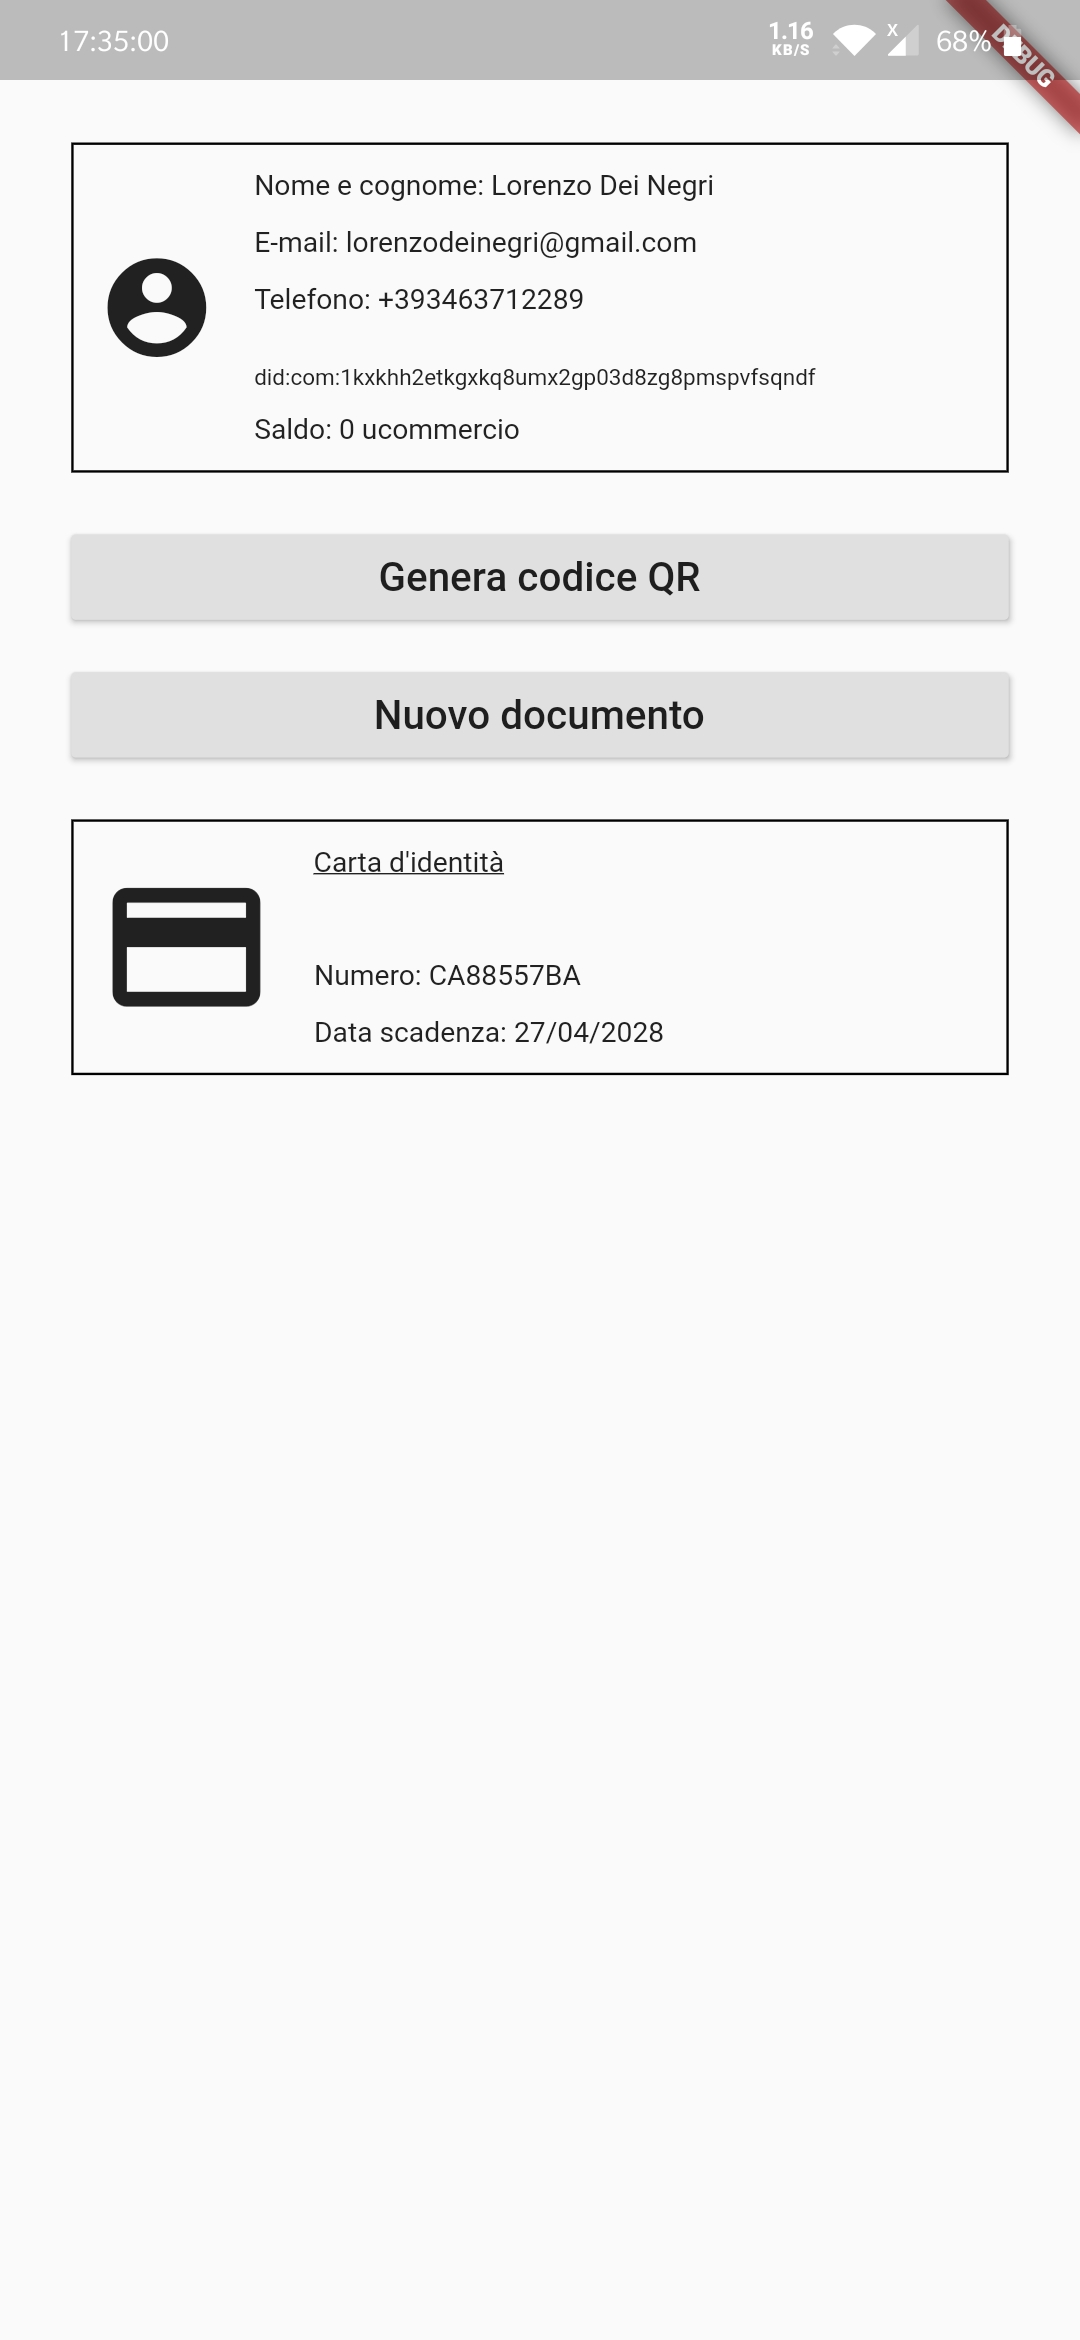
\includegraphics[height=\textheight]{home} 
	\caption{\textit{Layout} della classe Home}
\end{figure}

\subsubsection*{Login}

In questo \gls{namespaceg} sono raggruppate tutte le classi utilizzate per la realizzazione delle schermate che permettono all'utente di effettuare l'accesso all'applicazione.

\begin{namespacedesc}
	\classdesc{Login}{la classe Login implementa un componente grafico senza mantenimento di stato con due pulsanti per scegliere se proseguire con il recupero di un'identità digitale precedentemente creata su un dispositivo differente oppure se crearne una nuova. Nel caso fosse già stata creata un'identità sul dispositivo corrente il componente grafico chiederà automaticamente all'utente di autenticarsi: se questi ha scelto l'autenticazione biometrica apparirà la richiesta di sistema e, se il controllo viene superato, viene istanziato e mostrato un componente grafico di classe Home, se invece l'utente ha scelto l'autenticazione tramite \textit{password} allora viene istanziato e mostrato un componente grafico di classe PasswordAuthentication.}
	
	\classdesc{PasswordAuthentication}{la classe PasswordAuthentication implementa un componente grafico con mantenimento di stato con un campo di testo per l'inserimento della \textit{password} utilizzata per accedere all'applicazione da parte di un utente registrato; inoltre sono presenti due pulsanti, per tornare alla schermata precedente oppure passare a quella successiva. Quando l'utente preme il pulsante per avanzare viene effettuato un controllo per verificare che la \textit{password} inserita sia la stessa memorizzata nel \textit{database} locale per l'utente di quel dispositivo, nel caso questo controllo venga superato allora viene istanziato e mostrato il componente grafico della schermata successiva, ossia la schermata di classe Home, altrimenti viene semplicemente mostrato un errore a schermo.}
\end{namespacedesc}

\newpage

\begin{figure}[H] 
	\centering 
	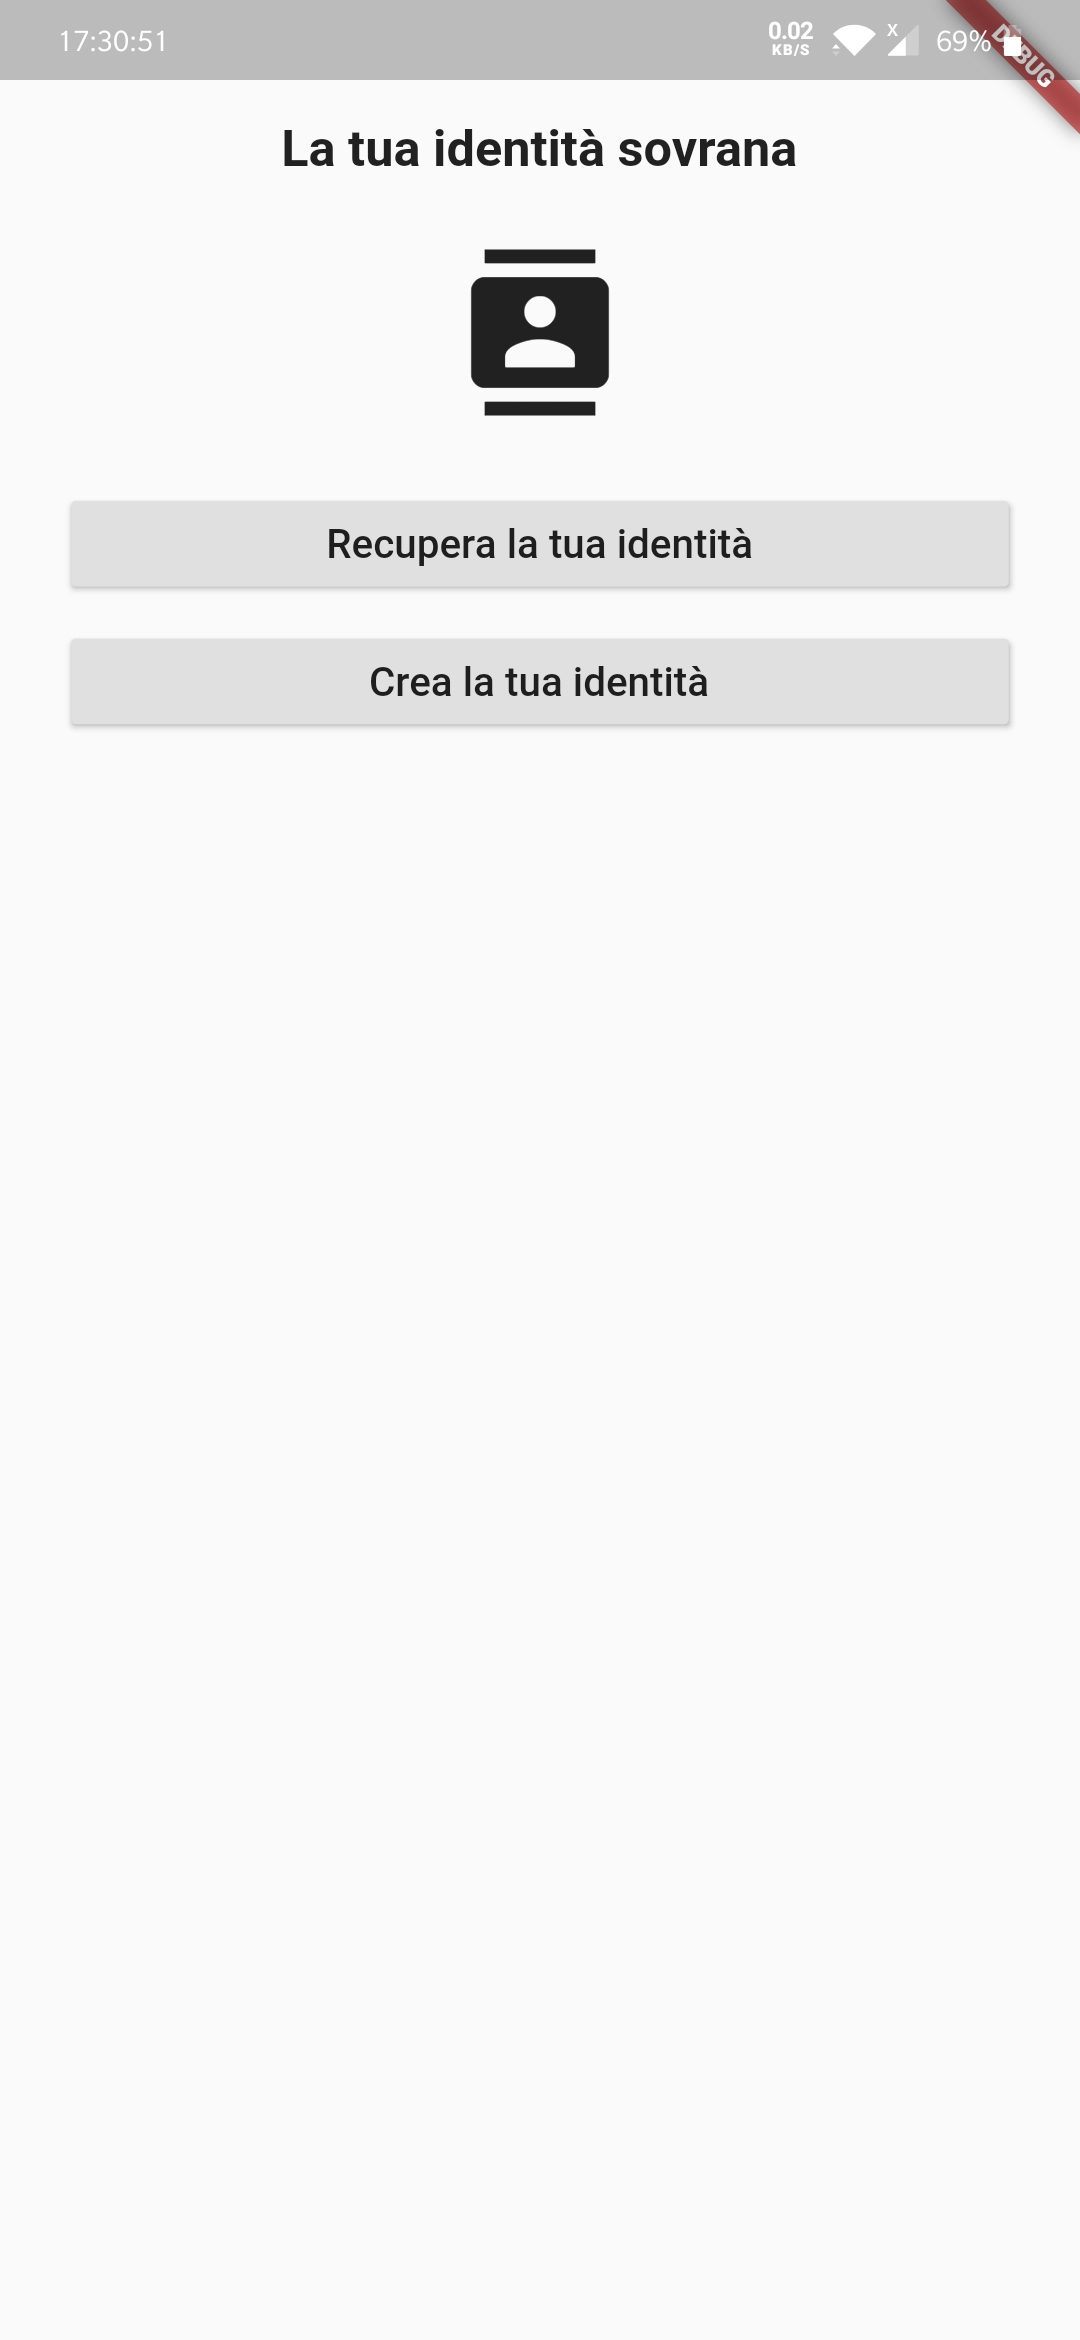
\includegraphics[height=\textheight]{login} 
	\caption{\textit{Layout} della classe Login}
\end{figure}

\subsubsection*{Recover}

In questo \gls{namespaceg} sono raggruppate tutte le classi utilizzate per la realizzazione delle schermate che permettono all'utente di seguire la procedura di recupero di un'identità digitale creata con un dispositivo mobile diverso da quello corrente.

\begin{namespacedesc}
	\classdesc{Authentication}{la classe Authentication implementa un componente grafico con mantenimento di stato con due pulsanti per scegliere la modalità di accesso durante il recupero dell'identità precedentemente creata su un altro dispositivo. I pulsanti permettono la scelta tra una \textit{password} alfanumerica e i sensori biometrici del dispositivo. Se viene scelta la seconda opzione il componente grafico mostra la richiesta di sistema attraverso la quale viene chiesto all'utente di autenticarsi e solamente dopo aver superato il controllo biometrico l'utente può proseguire. Se invece viene scelta la \textit{password} allora viene istanziato e mostrato un componente grafico di classe recover.Password.}
	
	\classdesc{recover.Password}{la classe recover.Password implementa un componente grafico con mantenimento di stato con due campi di testo per l'inserimento della \textit{password} da utilizzare, durante il recupero dell'identità precedentemente creata su un altro dispositivo, per accedere all'applicazione all'avvio successivo; inoltre sono presenti due pulsanti, per tornare alla schermata precedente oppure passare a quella successiva. Quando l'utente preme il pulsante per avanzare viene effettuato un controllo per validare la \textit{password} inserita, nel caso questo venga superato allora viene istanziato e mostrato il componente grafico della schermata successiva, altrimenti viene semplicemente mostrato un errore a schermo.}
	
	\classdesc{recover.Seed}{la classe recover.Seed implementa un componente grafico con mantenimento di stato con una casella di testo per consentire all'utente l'inserimento del codice mnemonico, utile per poter recuperare l'identità creata su un dispositivo differente da quello attualmente utilizzato; inoltre sono presenti due pulsanti, per tornare alla schermata precedente oppure passare a quella successiva. Quando l'utente preme il pulsante per avanzare viene effettuato un controllo per validare il codice mnemonico inserito, nel caso questo venga superato allora viene istanziato e mostrato il componente grafico della schermata successiva, ossia la schermata di classe Home, altrimenti viene semplicemente mostrato un errore a schermo.}
\end{namespacedesc}

\newpage

\begin{figure}[H] 
	\centering 
	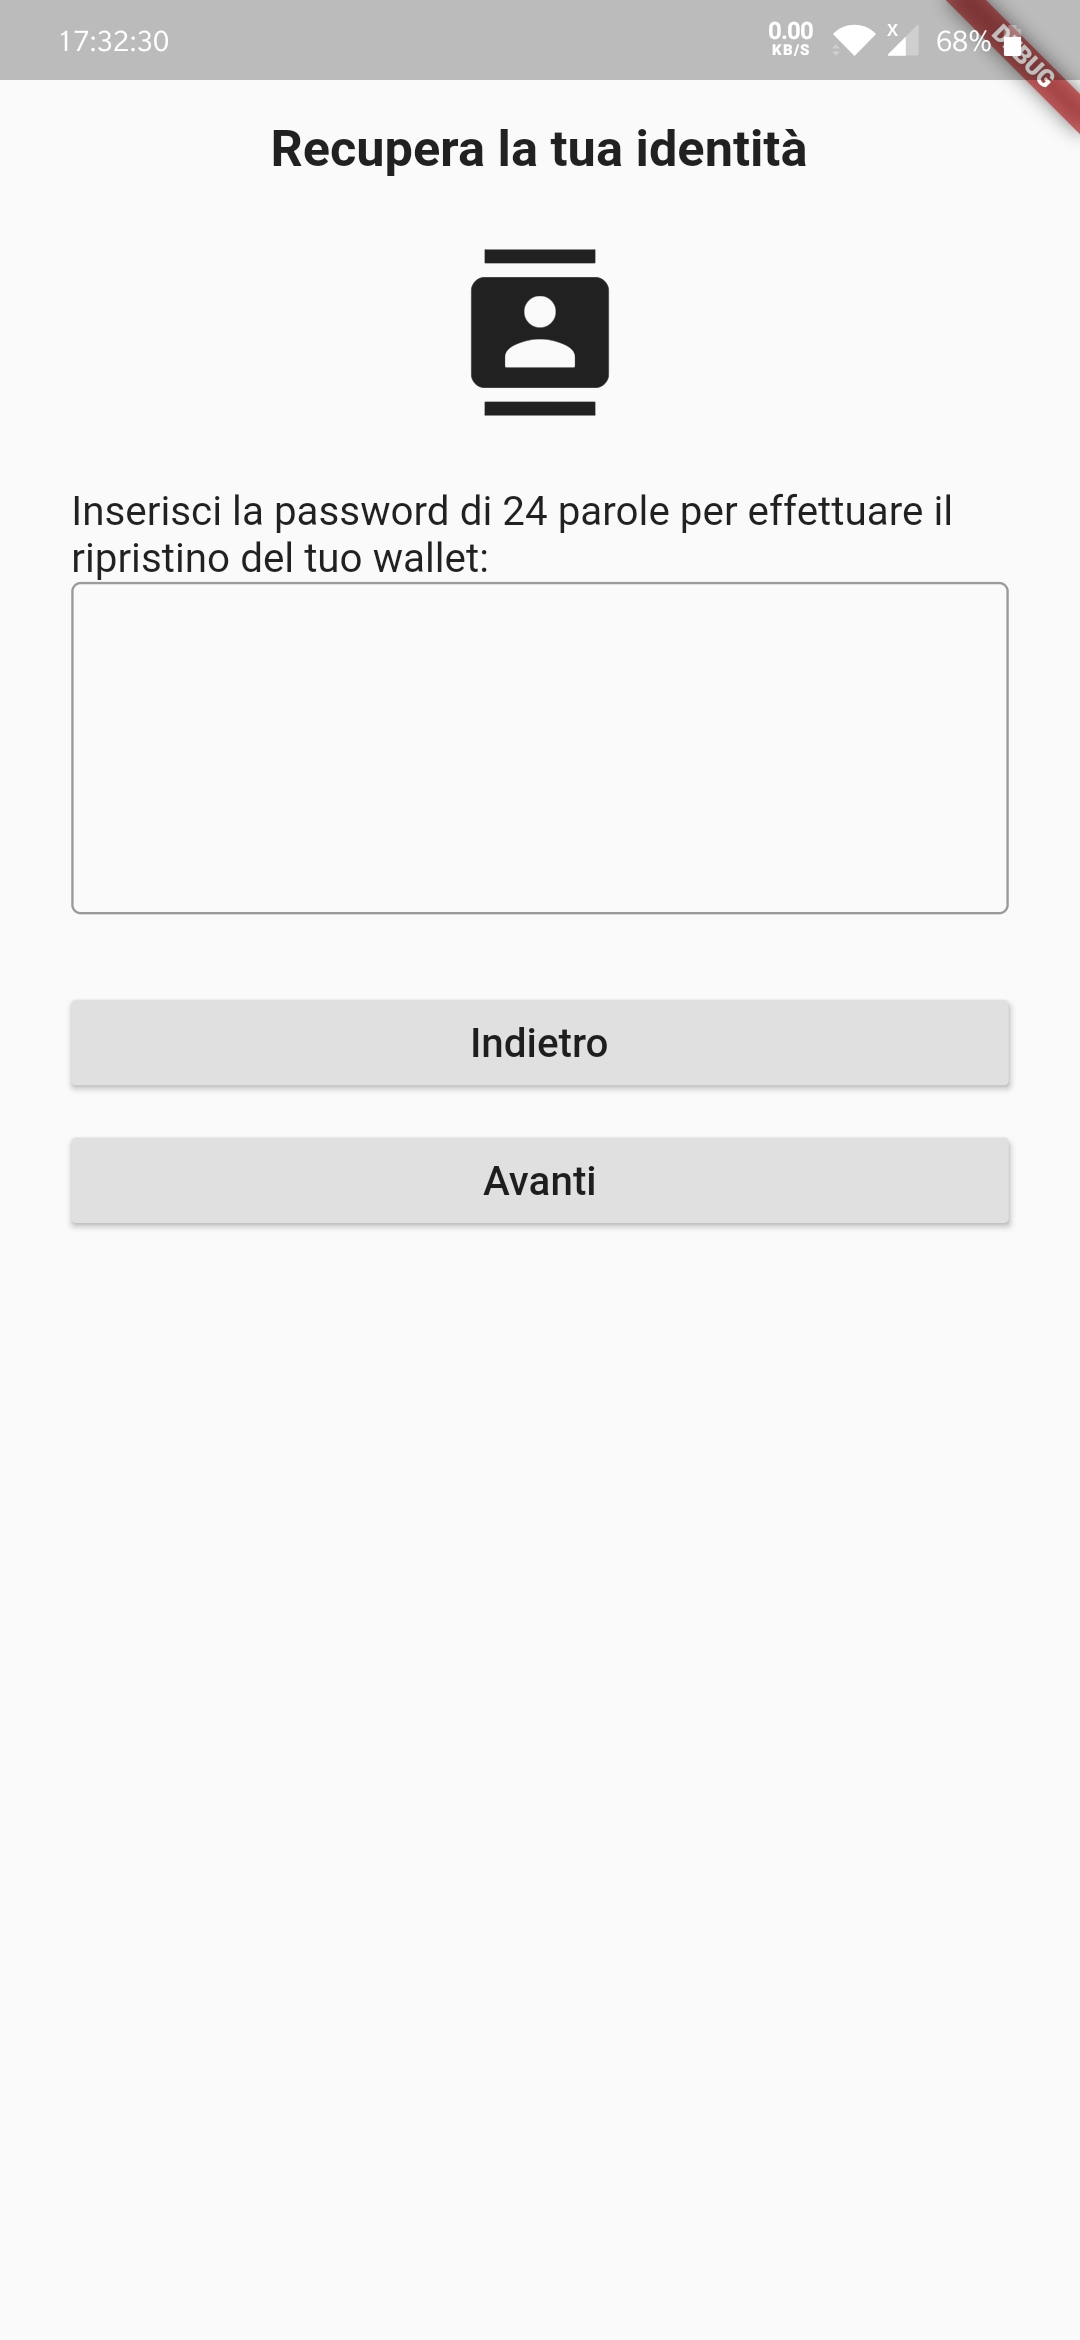
\includegraphics[height=\textheight]{login-seed} 
	\caption{\textit{Layout} della classe recover.Seed}
\end{figure}

\subsubsection*{Registration}

In questo \gls{namespaceg} sono raggruppate tutte le classi utilizzate per la realizzazione delle schermate che permettono all'utente di seguire la procedura di registrazione di una nuova identità digitale da utilizzare poi all'interno dell'applicazione.

\begin{namespacedesc}
	\classdesc{Email}{la classe Email implementa un componente grafico con mantenimento di stato con due campi di testo per l'inserimento della \textit{email} dell'utente che sta registrando una nuova identità digitale; inoltre sono presenti due pulsanti, per tornare alla schermata precedente oppure passare a quella successiva. Quando l'utente preme il pulsante per avanzare viene effettuato un controllo per validare l'\textit{email} inserita, nel caso questo venga superato allora viene istanziato e mostrato il componente grafico della schermata successiva, altrimenti viene semplicemente mostrato un errore a schermo.}
	
	\classdesc{EmailConfirm}{la classe EmailConfirm implementa un componente grafico con mantenimento di stato con una casella di testo in cui inserire il codice di verifica inviato per \textit{email} all'indirizzo inserito in precedenza, in modo da garantire che sia di proprietà dell'utente che sta registrando la propria identità tramite l'applicazione; inoltre è presente un \textit{link} per richiedere l'invio di un nuovo codice di verifica e due pulsanti, per tornare alla schermata precedente oppure passare a quella successiva. Quando l'utente preme il pulsante per avanzare viene effettuato un controllo per verificare che il codice di verifica inserito sia lo stesso inviato all'indirizzo \textit{email} dell'utente, nel caso questo controllo venga superato allora viene istanziato e mostrato il componente grafico della schermata successiva, altrimenti viene semplicemente mostrato un errore a schermo.}
	
	\classdesc{Generality}{la classe Generality implementa un componente grafico con mantenimento di stato con due caselle di testo per l'inserimento del nome e del cognome dell'utente che sta registrando una nuova identità digitale; inoltre sono presenti due pulsanti per scegliere la modalità di accesso all'applicazione una volta completata la procedura di registrazione. I pulsanti permettono la scelta tra una \textit{password} alfanumerica e i sensori biometrici del dispositivo. Se viene scelta la seconda opzione il componente grafico mostra la richiesta di sistema attraverso la quale viene chiesto all'utente di autenticarsi e solamente dopo aver superato il controllo biometrico l'utente può proseguire. Se invece viene scelta la \textit{password} allora viene istanziato e mostrato un componente grafico di classe registration.Password.\\
	Prima di procedere con il controllo dei dati biometrici o con la visualizzazione del componente grafico per l'inserimento della \textit{password} viene effettuato un controllo per validare la il nome e il cognome inseriti, solo nel caso questo venga superato allora si procedere con quanto descritto in precedenza, altrimenti viene semplicemente mostrato un errore a schermo.}
	
	\classdesc{registration.Password}{la classe registration.Password implementa un componente grafico con mantenimento di stato con due campi di testo per l'inserimento della \textit{password} da utilizzare per accedere all'applicazione una volta completata la procedura di registrazione; inoltre sono presenti due pulsanti, per tornare alla schermata precedente oppure passare a quella successiva. Quando l'utente preme il pulsante per avanzare viene effettuato un controllo per validare la \textit{password} inserita, nel caso questo venga superato allora viene istanziato e mostrato il componente grafico della schermata successiva, altrimenti viene semplicemente mostrato un errore a schermo.}
	
	\classdesc{Phone}{la classe Phone implementa un componente grafico con mantenimento di stato con due campi di testo per l'inserimento del numero di telefono dell'utente che sta registrando una nuova identità digitale; inoltre sono presenti due pulsanti, per tornare alla schermata precedente oppure passare a quella successiva. Quando l'utente preme il pulsante per avanzare viene effettuato un controllo per validare il numero di telefono inserito, nel caso questo venga superato allora viene istanziato e mostrato il componente grafico della schermata successiva, altrimenti viene semplicemente mostrato un errore a schermo.}
	
	\classdesc{PhoneConfirm}{la classe PhoneConfirm implementa un componente grafico con mantenimento di stato con una casella di testo in cui inserire il codice di verifica inviato tramite \gls{sms} al numero di telefono inserito in precedenza, in modo da garantire che sia di proprietà dell'utente che sta registrando la propria identità tramite l'applicazione; inoltre è presente un \textit{link} per richiedere l'invio di un nuovo codice di verifica e due pulsanti, per tornare alla schermata precedente oppure passare a quella successiva. Quando l'utente preme il pulsante per avanzare viene effettuato un controllo per verificare che il codice di verifica inserito sia lo stesso inviato al numero di telefono dell'utente, nel caso questo controllo venga superato allora viene istanziato e mostrato il componente grafico della schermata successiva, altrimenti viene semplicemente mostrato un errore a schermo.}
	
	\classdesc{registration.Seed}{la classe registration.Seed implementa un componente grafico senza mantenimento di stato con una casella di testo contenente il codice mnemonico, utile per poter generare il \gls{walletg} associato all'identità creata sul dispositivo utilizzato; inoltre sono presenti tre pulsanti: per salvare il codice in formato \gls{pdf} sul dispositivo, per stamparlo tramite una stampante presente nella stessa rete locale del dispositivo e per passare alla schermata successiva. Quando l'utente preme il pulsante per avanzare viene generato il \gls{walletg} a partire dal codice visto in precedenza, da quel momento in poi non è più possibile reperire il codice mnemonico e viene istanziato e mostrato il componente grafico della schermata successiva, ossia la schermata di classe Home.}
\end{namespacedesc}

\newpage

\begin{figure}[H] 
	\centering 
	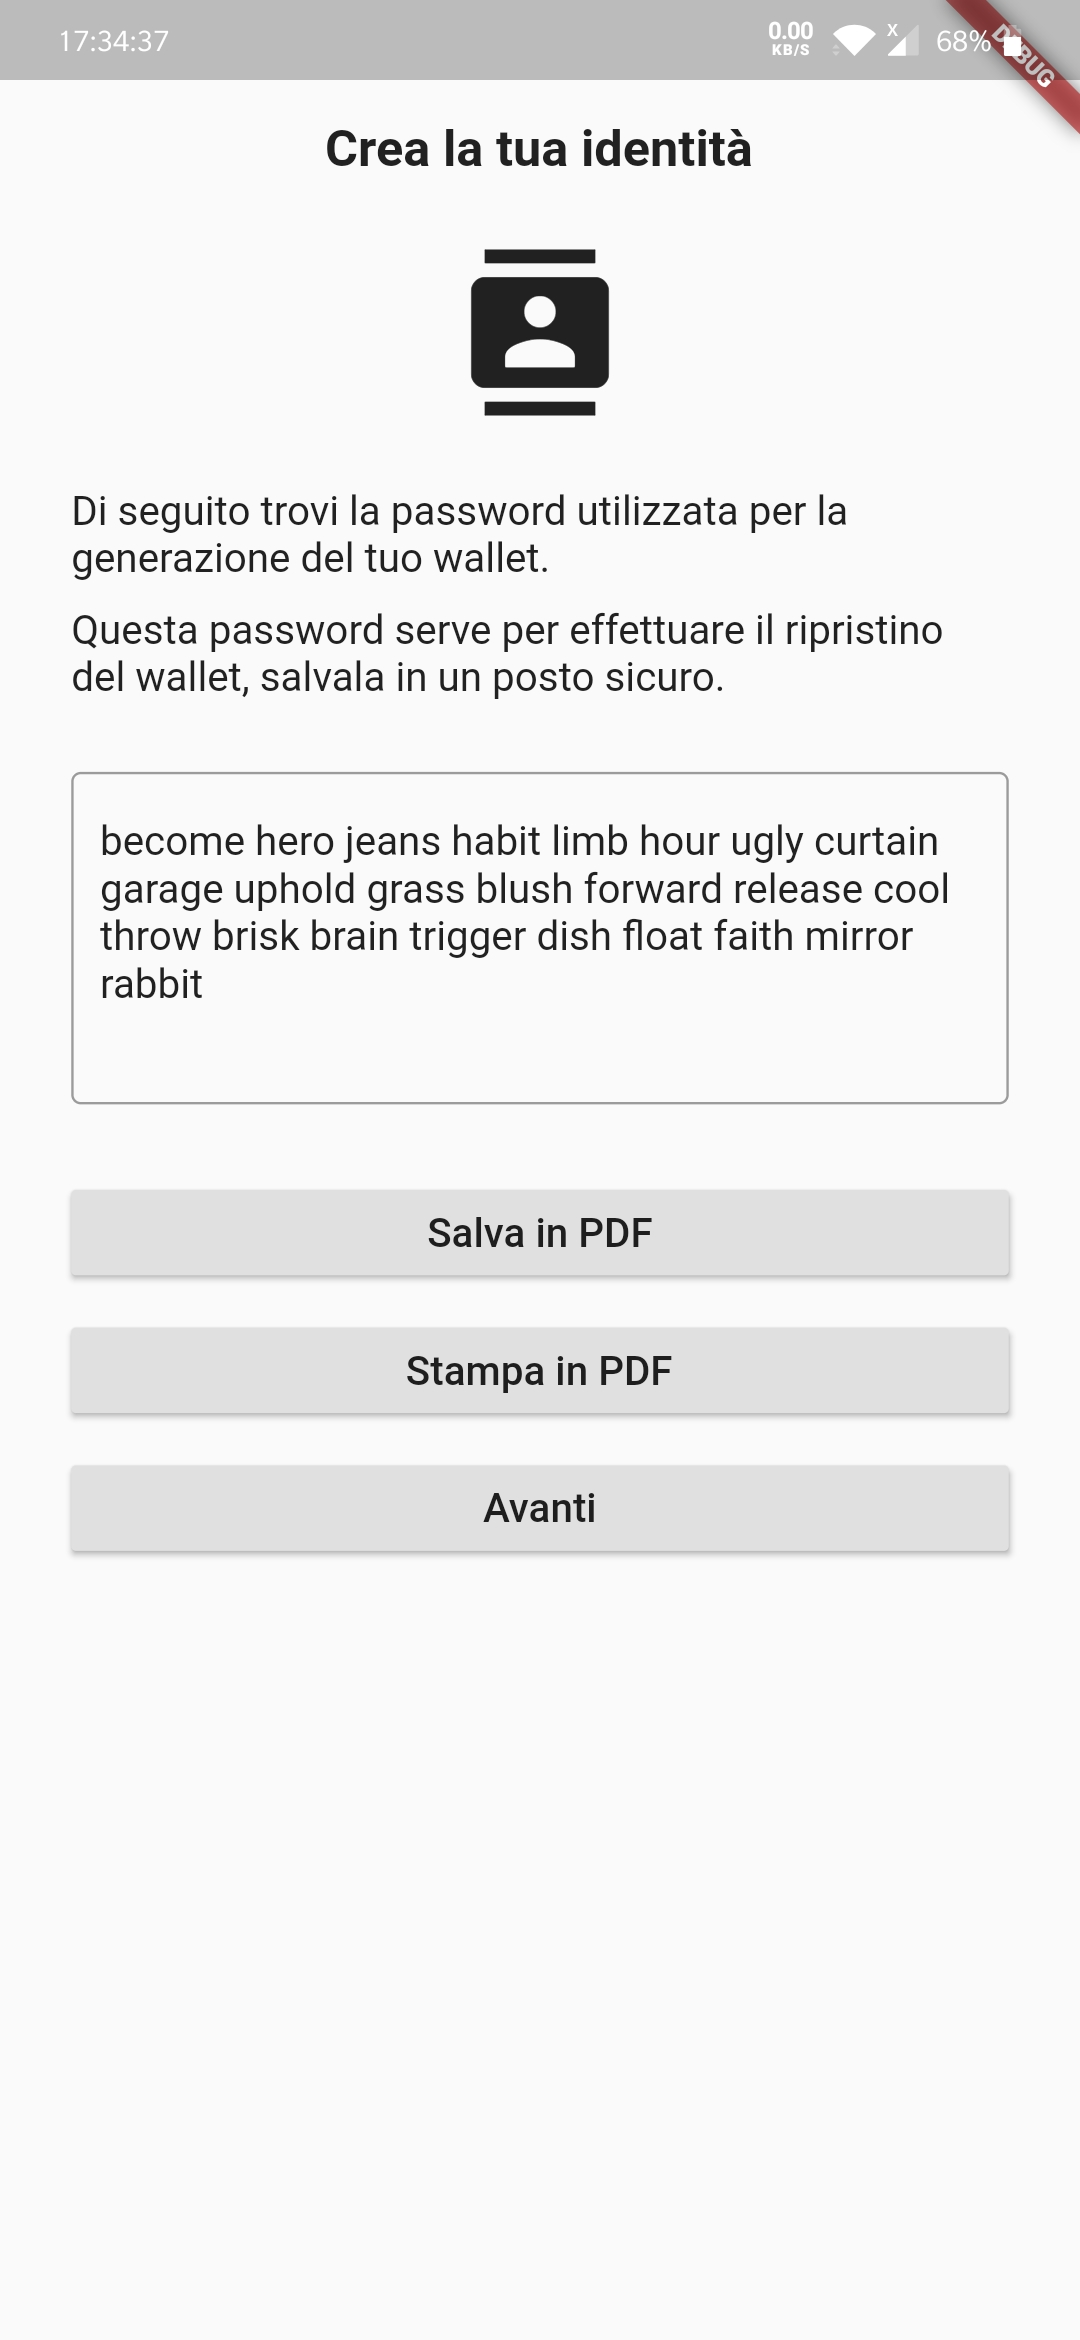
\includegraphics[height=\textheight]{registration-seed} 
	\caption{\textit{Layout} della classe registration.Seed}
\end{figure}

%**************************************************************
\section{Codifica}

Tutta l'applicazione, compresa l'interfaccia grafica, è stata sviluppata utilizzando il linguaggio di programmazione Dart, tramite il quale sono state implementate tutte le classi previste durante la progettazione. Questo è stato possibile grazie alle funzionalità del \gls{frameworkg} Flutter, il quale mette a disposizione degli sviluppatori delle classi che realizzano ciascuna un componente grafico con una funzione specifica. Quindi, per creare le schermate dell'applicazione è stato sufficiente realizzare una singola classe per ognuna di esse, estendendo un'apposita superclasse comune a tutte le classi fornite da Flutter; all'interno dei metodi di costruzione e renderizzazione derivati sono stati poi composti tra di loro tutti gli opportuni oggetti, istanziandone uno dentro l'altro e valorizzandone i vari attributi utili a formare il \textit{layout} desiderato.\\
Per l'implementazione di alcune funzionalità e/o di alcuni componenti grafici specifici sono stati utilizzati dei pacchetti esterni che rispondessero a tali esigenze, questi sono stati aggiunti come dipendenze del progetto tramite un apposito \textit{file} di configurazione fornito dal \gls{frameworkg}. Infatti, Flutter mette a disposizione un meccanismo che si occupa di gestire l'importazione e l'aggiornamento di tutte le estensioni utilizzate dal progetto tramite dei semplici comandi eseguibili attraverso un terminale.\\ 
Alcuni di questi pacchetti sono stati utilizzati anche nell'implementazione delle classi che realizzano la logica applicativa, in particolare sono state necessarie le librerie sviluppare da Commerc.io S.r.l. per permettere l'interazione con la \gls{blockchaing}. Ogni classe di interesse fornita è stata opportunamente incapsulata all'interno di un'altra classe realizzata \textit{ad hoc} per estenderne e raffinarne le funzionalità.

%**************************************************************
\section{Test}

Data la natura di \gls{poc} dell'applicazione, \myCompany{} \companyTitle{} non ha ritenuto fosse di suo interesse la realizzazione di specifici test automatici che ne garantissero la corretta esecuzione. L'azienda ha richiesto solamente una dimostrazione pratica del funzionamento di tutte le funzionalità più significative implementate, in quanto l'obiettivo principale era dimostrare la fattibilità del progetto aziendale con il quale punta a gestire, sia le \gls{ssi} che i documenti firmati, in modo completo, tramite un'unica applicazione utilizzabile in ogni tipologia di sistema.\\
Di conseguenza, durante tutto lo sviluppo, di ogni nuova funzionalità implementata ne veniva provato manualmente il funzionamento prima di procedere con quella successiva. Poi, man mano che veniva realizzata l'interfaccia grafica, testandone il comportamento venivano anche riprovate tutte le funzioni della logica applicativa coinvolte nelle operazioni svolte. Infine, al termine dello sviluppo, assieme al tutor aziendale, è stato fatto un test generale che comprendesse ogni singola funzionalità esposta dall'interfaccia.

%**************************************************************
\section{Valutazioni}

Il risultato ottenuto al termine dello sviluppo dell'applicazione è stato valutato molto positivamente da parte dell'azienda, in quanto il \textit{software} funziona correttamente, ha il comportamento atteso e sono state realizzate tutte le funzionalità di interesse per il progetto aziendale. Inoltre, grazie alla bontà dei risultati delle attività di analisi e progettazione, è stato possibile rendere disponibili ulteriori operazioni di importanza secondaria, il che ha permesso di ottenere un prodotto che va oltre le aspettative iniziali di \myCompany{} \companyTitle{}.\\
Infatti, il lavoro svolto ha portato al soddisfacimento di tutti i requisiti obbligatori e facoltativi; tra quelli desiderabili, gli unici rimasti incompiuti sono quelli riguardanti l'inserimento di un documento all'interno dell'applicazione. Tuttavia la funzionalità non risulta essere assente, ma soltanto incompleta: sono stati implementati e testati tutti i relativi metodi della logica applicativa però, per motivi di tempo, non è stato possibile realizzare l'interfaccia grafica delle schermate che ne avrebbero permesso l'utilizzo da parte degli utenti.\\
Di seguito viene riportato lo stato di tutti i requisiti al termine dello sviluppo del \gls{poc}, suddivisi in tre tabelle, una per ogni tipologia.

\rowcolors{1}{grayer}{white}
\begin{longtable}{|c|p{7.65cm}|c|}
	\hline
	\rowcolor{gray}
	\textbf{Requisito} & \textbf{Descrizione} & \textbf{Stato} \\
	\hline
	RFO-1     & L'applicazione deve permettere l'inserimento del nome dell'utente. & Soddisfatto \\
	\hline
	RFO-2     & L'applicazione deve permettere l'inserimento del cognome dell'utente. & Soddisfatto \\
	\hline
	RFO-3     & L'applicazione deve permettere l'inserimento dell'indirizzo di posta elettronica dell'utente. & Soddisfatto \\
	\hline
	RFO-4     & L'applicazione deve permettere l'inserimento del numero di telefono cellulare dell'utente. & Soddisfatto \\
	\hline
	RFO-5     & L'applicazione deve permettere l'inserimento del codice di verifica dell'indirizzo di posta elettronica dell'utente. & Soddisfatto \\
	\hline
	RFO-6     & L'applicazione deve permettere l'inserimento del codice di verifica del numero di telefono cellulare dell'utente. & Soddisfatto \\
	\hline
	RFO-7     & L'applicazione deve permettere l'invio del codice di verifica dell'indirizzo di posta elettronica dell'utente. & Soddisfatto \\
	\hline
	RFO-8     & L'applicazione deve permettere l'invio del codice di verifica del numero di telefono cellulare dell'utente. & Soddisfatto \\
	\hline
	RFO-9     & L'applicazione deve permettere la visualizzazione del codice mnemonico. & Soddisfatto \\
	\hline
	RFO-10    & L'applicazione deve permettere l'inserimento del codice mnemonico. & Soddisfatto \\
	\hline
	RFO-11    & L'applicazione deve permettere l'inserimento di una \textit{password} per l'accesso da parte dell'utente. & Soddisfatto \\
	\hline
	RFO-12    & L'applicazione deve permettere l'inserimento della \textit{password} di accesso dell'utente. & Soddisfatto \\
	\hline
	RFO-13    & L'applicazione deve permettere la scelta dell'accesso tramite \textit{password} da parte dell'utente. & Soddisfatto \\
	\hline
	RFO-14    & L'applicazione deve permettere l'inserimento della password per l'accesso da parte dell'utente. & Soddisfatto \\
	\hline
	RFO-15    & L'applicazione deve permettere la visualizzazione del nome dell'utente. & Soddisfatto \\
	\hline
	RFO-16    & L'applicazione deve permettere la visualizzazione del cognome dell'utente. & Soddisfatto \\
	\hline
	RFO-17    & L'applicazione deve permettere la visualizzazione dell'indirizzo di posta elettronica dell'utente. & Soddisfatto \\
	\hline
	RFO-18    & L'applicazione deve permettere la visualizzazione del numero di telefono cellulare dell'utente. & Soddisfatto \\
	\hline
	RFO-19    & L'applicazione deve permettere la visualizzazione dell'indirizzo pubblico del \gls{walletg} dell'utente. & Soddisfatto \\
	\hline
	RFO-20    & L'applicazione deve permettere la visualizzazione del saldo del \gls{walletg} dell'utente. & Soddisfatto \\
	\hline
	RFO-21    & L'applicazione deve permettere la visualizzazione della foto profilo dell'utente. & Soddisfatto \\
	\hline
	RFO-22    & L'applicazione deve permettere la visualizzazione della lista dei documenti inseriti dall'utente. & Soddisfatto \\
	\hline
	RFO-23    & L'applicazione deve permettere la registrazione di una nuova identità da parte dell'utente. & Soddisfatto \\
	\hline
	RFO-24    & L'applicazione deve permettere il recupero di un'identità creata in precedenza da parte dell'utente. & Soddisfatto \\
	\hline
	RFO-25    & L'applicazione deve permettere l'accesso tramite autenticazione da parte dell'utente. & Soddisfatto \\
	\hline
	RFD-1     & L'applicazione deve permettere il reinvio del codice di verifica dell'indirizzo di posta elettronica dell'utente. & Soddisfatto \\
	\hline
	RFD-2     & L'applicazione deve permettere il reinvio del codice di verifica del numero di telefono cellulare dell'utente. & Soddisfatto \\
	\hline
	RFD-3     & L'applicazione deve permettere il salvataggio del codice mnemonico in formato \gls{pdf}. & Soddisfatto \\
	\hline
	RFD-4     & L'applicazione deve permettere la scelta dell'accesso tramite dati biometrici da parte dell'utente. & Soddisfatto \\
	\hline
	RFD-5     & L'applicazione deve permettere l'inserimento dei dati biometrici per l'accesso da parte dell'utente. & Soddisfatto \\
	\hline
	RFD-6     & L'applicazione deve permettere l'inserimento della foto profilo da parte dell'utente. & Soddisfatto \\
	\hline
	RFD-7     & L'applicazione deve permettere l'inserimento del titolo di un documento da parte dell'utente. & Non soddisfatto \\
	\hline
	RFD-8     & L'applicazione deve permettere l'inserimento delle informazioni di un documento da parte dell'utente. & Non soddisfatto \\
	\hline
	RFD-9     & L'applicazione deve permettere l'inserimento di un documento da parte dell'utente. & Non soddisfatto \\
	\hline
	RFF-1     & L'applicazione deve permettere la stampa del codice mnemonico. & Soddisfatto \\
	\hline
	RFF-2     & L'applicazione deve permettere la visualizzazione del codice QR associato all'indirizzo pubblico del \gls{walletg}. & Soddisfatto \\
	\hline
	RFF-3     & L'applicazione deve permettere la modifica della foto profilo da parte dell'utente. & Soddisfatto \\
	\hline
	RFF-4     & L'applicazione deve permettere l'inserimento della foto di un documento da parte dell'utente. & Soddisfatto \\
	\hline
	
	\caption{Tabella dello stato dei requisti funzionali}
	\label{tab:stato-requisiti-funzionali}
\end{longtable}

\rowcolors{1}{white}{grayer}
\begin{longtable}{|c|p{8.35cm}|c|}
	\hline
	\rowcolor{gray}
	\textbf{Requisito} & \textbf{Descrizione} & \textbf{Stato} \\
	\hline
	RQO-1    & Deve essere fornita una documentazione delle procedure di installazione e configurazione di tutte le tecnologie e gli strumenti utilizzati per sviluppare e testare l'applicazione. & Soddisfatto \\
	\hline
	RQO-2    & Deve essere fornita una documentazione di tutte le classi che compongono l'applicazione, con i relativi metodi. & Soddisfatto \\
	\hline
	RQO-3    & Il processo di sviluppo deve fare uso di un sistema di versionamento. & Soddisfatto \\
	\hline
	
	\caption{Tabella dello stato dei requisiti qualitativi}
	\label{tab:stato-requisiti-qualitativi}
\end{longtable}

\rowcolors{1}{white}{grayer}
\begin{longtable}{|c|p{8.35cm}|c|}
	\hline
	\rowcolor{gray}
	\textbf{Requisito} & \textbf{Descrizione} & \textbf{Stato} \\
	\hline
	RVO-1    & L'applicazione deve essere scritta utilizzando il linguaggio Dart. & Soddisfatto \\
	\hline
	RVO-2    & L'applicazione deve essere scritta utilizzando il \gls{frameworkg} Flutter. & Soddisfatto \\
	\hline
	RVO-3    & L'applicazione deve interagire con la \gls{blockchaing} della \textit{Commercio.network}. & Soddisfatto \\
	\hline
	RVO-4    & L'interazione a basso livello con la \gls{blockchaing} deve avvenire tramite la libreria Sacco, sviluppata da Commerc.io S.r.l. per il linguaggio di programmazione Dart. & Soddisfatto \\
	\hline
	RVO-5    & L'interazione ad alto livello con la \gls{blockchaing} deve avvenire tramite la libreria CommercioSDK, sviluppata da Commerc.io S.r.l. per il linguaggio di programmazione Dart. & Soddisfatto \\
	\hline
	RVO-6    & L'applicazione deve essere eseguibile su sistema operativo Android. & Soddisfatto \\
	\hline
	RVD-1    & L'applicazione deve essere eseguibile su sistema operativo iOS. & Soddisfatto \\
	\hline
	
	\caption{Tabella dello stato dei requisiti di vincolo}
	\label{tab:stato-requisiti-vincolo}
\end{longtable}

L'applicazione, per quanto sia soltanto un \gls{poc} e quindi lontano dall'essere compiuta, può essere una base valida su cui l'azienda potrà costruire il \textit{software} completo che intende sviluppare. Infatti è stata progettata per essere facilmente estendibile sia in ampiezza, aggiungendo nuove funzionalità, che in profondità, raffinando quelle già esistenti. 